\documentclass[10pt]{beamer}

%\usepackage[utf8]{inputenc}
\usepackage[spanish]{babel} % Español
\usepackage{graphicx}
\usepackage{tabularx} % Tablas ajustables
\usepackage{booktabs}
\usepackage{adjustbox}
\usepackage{bm}
\usepackage{mathtools}
\usepackage{utopia} % Fuente Utopia
\usepackage{caption}
\usepackage{natbib}
\usepackage{hyperref}

\usetheme{Madrid}
\usefonttheme{professionalfonts}
% Colores
\definecolor{myNewColorA}{RGB}{139,0,0}
\definecolor{myNewColorB}{RGB}{139,0,0}
\definecolor{myNewColorC}{RGB}{139,0,0}
\setbeamercolor*{palette primary}{bg=myNewColorC}
\setbeamercolor*{palette secondary}{bg=myNewColorB, fg = white}
\setbeamercolor*{palette tertiary}{bg=myNewColorA, fg = white}
\setbeamercolor*{titlelike}{fg=myNewColorA}
\setbeamercolor*{title}{bg=myNewColorA, fg = white}
\setbeamercolor*{item}{fg=myNewColorA}
\setbeamercolor*{caption name}{fg=myNewColorA}

% Fuentes de portada
\setbeamerfont{title}{size=\large}
\setbeamerfont{subtitle}{size=\small}
\setbeamerfont{author}{size=\small}
\setbeamerfont{date}{size=\small}
\setbeamerfont{institute}{size=\small}


% Título y portada
\title[Sección 4]{La brecha salario-genero}
\author[Grupo 3]{Catalina Leal Rojas, Lucas Daniel Carrillo Aguirre, Lucas Eduardo Veras Costa, Maria Paula Basto Lozano}

% Espacio para el logo en la portada
\titlegraphic{\vspace{1cm}
\includegraphics[width=2.5cm]{../../views/logo.png}}

\setbeamertemplate{navigation symbols}{}

\begin{document}

% Portada
\frame{\titlepage}
%---------------------------------------------------------------------------
%---------------- SLIDE 1 ----------------
\begin{frame}{Brecha género-salario: introducción}
\begin{itemize}
    \item Analizamos la relación entre género e ingresos.
    \item Medida clave: \textbf{salario por hora}, permite aislar el efecto de las horas trabajadas.
    \item Se emplea el \textbf{logaritmo del ingreso}, lo que facilita la interpretación en términos porcentuales.
    \item Se consideran únicamente individuos ocupados.
\end{itemize}

\[
\log(\omega) = \beta_0 + \beta_1 Female + u
\]

\begin{center}
\resizebox{0.9\textwidth}{!}{%
\begin{tabular}{@{\extracolsep{5pt}}lccccc}  
\\[-1.8ex]\hline 
\hline \\[-1.8ex] 
 & log(ysalarym) & log(ysalarymha) & log(yingLabm) & log(ytotalm) & log(ytotalmha) \\  
 & (1) & (2) & (3) & (4) & (5) \\  
\hline \\[-1.8ex] 
female & $-$0.149$^{***}$ & $-$0.045$^{***}$ & $-$0.147$^{***}$ & $-$0.238$^{***}$ & $-$0.090$^{***}$ \\    
 & (0.015) & (0.015) & (0.015) & (0.015) & (0.014) \\  
Constant & 13.977$^{***}$ & 8.641$^{***}$ & 14.088$^{***}$ & 13.981$^{***}$ & 8.667$^{***}$ \\    
 & (0.011) & (0.010) & (0.011) & (0.010) & (0.009) \\  
\hline \\[-1.8ex] 
Observaciones & 9,892 & 9,892 & 9,892 & 14,764 & 14,764 \\  
R$^{2}$ & 0.010 & 0.001 & 0.009 & 0.018 & 0.003 \\  
\hline 
\textit{Nota:} & \multicolumn{5}{r}{$^{*}$p$<$0.1; $^{**}$p$<$0.05; $^{***}$p$<$0.01} \\  
\end{tabular}  
} % cierre resizebox
\end{center}

\end{frame}

%---------------- SLIDE 2 ----------------
\begin{frame}{Teorema de FWL y bootstrap}
\begin{itemize}
    \item El Teorema de Frisch-Waugh-Lovell (FWL) permite aislar el efecto de una variable controlando por otras en tres pasos: 
    \begin{enumerate}
        \item Residuos de $y$ sobre controles.
        \item Residuos de $X_1$ sobre controles.
        \item Regresión de residuos: coeficiente idéntico al MCO.
    \end{enumerate}
    \item En nuestro caso, el coeficiente de $female$ por FWL coincide con el obtenido por MCO.
\end{itemize}

\vspace{0.3cm}

\centering
\scalebox{0.6}{ % ajustar tamaño para que quepa en la slide
\begin{tabular}{@{\extracolsep{5pt}}lcc} 
\\[-1.8ex]\hline 
\hline \\[-1.8ex] 
 & \multicolumn{2}{c}{\textit{Variable dependiente:}} \\ 
\cline{2-3} 
 & log(y\_ingLab\_m) & resid\_ing \\ 
 & (1) & (2)\\ 
\hline \\[-1.8ex] 
 female & $-$0.163$^{***}$ &  \\ 
  & (0.015) &  \\ 
 age & 0.091$^{***}$ &  \\ 
  & (0.004) &  \\ 
 age\_sqr & $-$0.001$^{***}$ &  \\ 
  & (0.00005) &  \\ 
 resid\_fem &  & $-$0.163$^{***}$ \\ 
  &  & (0.017) \\ 
 Constant & 12.338$^{***}$ & $-$0.000 \\ 
  & (0.071) & (0.007) \\ 
\hline \\[-1.8ex] 
Observations & 9,892 & 9,892 \\ 
R$^{2}$ & 0.069 & 0.012 \\ 
Adjusted R$^{2}$ & 0.069 & 0.012 \\ 
Residual Std. Error & 0.739 (df = 9888) & 0.739 (df = 9890) \\ 
F Statistic & 245.548$^{***}$ (df = 3; 9888) & 119.495$^{***}$ (df = 1; 9890) \\ 
\hline 
\hline \\[-1.8ex] 
\textit{Note:}  & \multicolumn{2}{r}{$^{*}$p$<$0.1; $^{**}$p$<$0.05; $^{***}$p$<$0.01} \\ 
\end{tabular} 
}

\vspace{0.3cm}

\begin{figure}
    \centering
    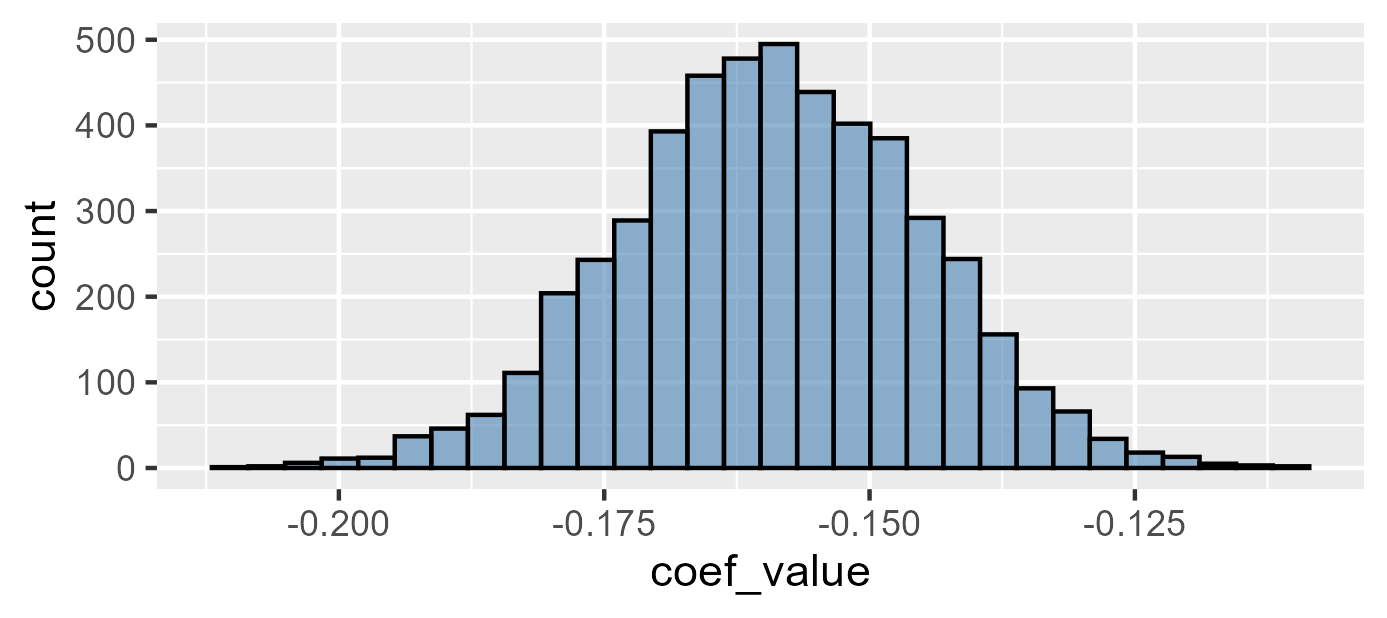
\includegraphics[scale=0.45]{../../views/sd_fwl_hist.png}
    \caption{Distribución bootstrap (5000 repeticiones) del coeficiente de $female$.}
\end{figure}
\end{frame}
%----------------------------------------------------------------------------------------
%---------------- SLIDE ----------------
\begin{frame}{Errores estándar y bootstrap}
\begin{itemize}
    \item El Cuadro anterior muestra que los coeficientes de $female$ y $resid\_fem$ son idénticos. 
    \item Sin embargo, los errores estándar no lo son. Esto ocurre porque en la segunda regresión se reducen las variables y, por ende, los grados de libertad.
    \item Otra manera de estimar el error estándar es mediante el \textbf{bootstrap}, que consiste en remuestrear la muestra muchas veces y recalcular el coeficiente.
    \item El error estándar se obtiene a partir de la dispersión de esta distribución de estimaciones.
\end{itemize}

\vspace{0.3cm}

\begin{figure}
    \centering
    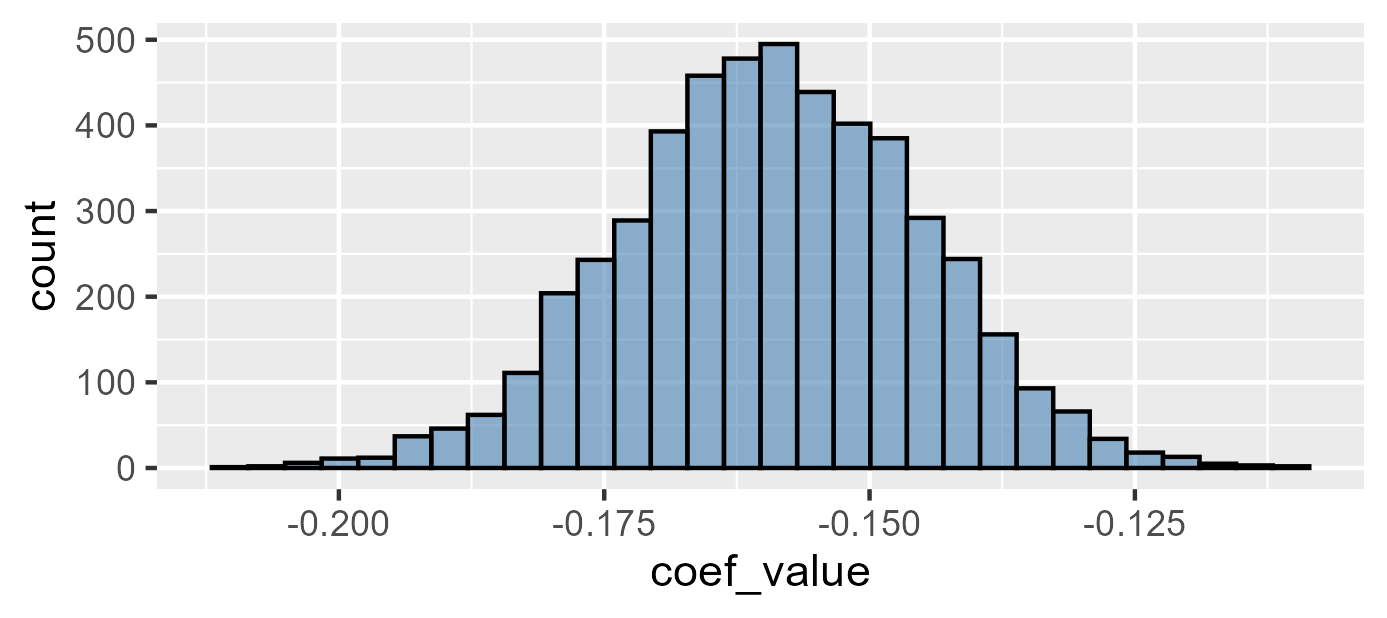
\includegraphics[scale=0.45]{../../views/sd_fwl_hist.png}
    \caption{Distribución bootstrap (5000 repeticiones) del coeficiente de $female$.}
\end{figure}

\end{frame}
%----------------------------------------------------------------------------------------

\begin{frame}{Controles y regresiones}
\begin{itemize}
    \item Se incluyen controles de:
    \begin{itemize}
        \item Capital humano (edad, educación).
        \item Intensidad laboral (horas, segundo empleo).
        \item Características del empleo (ocupación, formalidad, tamaño de firma).
    \end{itemize}
    \item Incluso con estos controles, el coeficiente de $female$ se mantiene \textbf{negativo y significativo}.
\end{itemize}

\begin{center}
\scalebox{0.55}{ % <-- ajusta el tamaño según espacio
\begin{tabular}{@{\extracolsep{5pt}}lccccc} 
\\[-1.8ex]\hline 
\hline \\[-1.8ex] 
 & \multicolumn{5}{c}{\textit{Dependent variable: log(y\_total\_m\_ha)}} \\ 
\cline{2-6} 
 & (1) & (2) & (3) & (4) & (5)\\ 
\hline \\[-1.8ex] 
 female & $-$0.043$^{***}$ & $-$0.056$^{***}$ & $-$0.137$^{***}$ & $-$0.173$^{***}$ & $-$0.101$^{***}$ \\ 
  & (0.014) & (0.014) & (0.011) & (0.011) & (0.011) \\ 
 age &  & 0.067$^{***}$ & 0.061$^{***}$ & 0.067$^{***}$ & 0.038$^{***}$ \\ 
  &  & (0.003) & (0.003) & (0.003) & (0.002) \\ 
 age\_sqr &  & $-$0.001$^{***}$ & $-$0.001$^{***}$ & $-$0.001$^{***}$ & $-$0.0004$^{***}$ \\ 
  &  & (0.00004) & (0.00004) & (0.00004) & (0.00003) \\ 
 as.factor(max\_educ\_level)3 &  &  & 0.199$^{**}$ & 0.222$^{**}$ & 0.167$^{**}$ \\ 
 as.factor(max\_educ\_level)4 &  &  & 0.288$^{***}$ & 0.301$^{***}$ & 0.203$^{***}$ \\ 
 as.factor(max\_educ\_level)5 &  &  & 0.340$^{***}$ & 0.348$^{***}$ & 0.224$^{***}$ \\ 
 as.factor(max\_educ\_level)6 &  &  & 0.552$^{***}$ & 0.561$^{***}$ & 0.285$^{***}$ \\ 
 as.factor(max\_educ\_level)7 &  &  & 1.216$^{***}$ & 1.202$^{***}$ & 0.540$^{***}$ \\ 
 total\_hours\_worked &  &  &  & $-$0.009$^{***}$ & $-$0.010$^{***}$ \\ 
 formal &  &  &  &  & 0.266$^{***}$ \\ 
 Constant & 8.735$^{***}$ & 7.410$^{***}$ & 6.623$^{***}$ & 6.969$^{***}$ & 8.342$^{***}$ \\ 
\hline \\[-1.8ex] 
Observations & 9,892 & 9,892 & 9,891 & 9,891 & 9,891 \\ 
R$^{2}$ & 0.001 & 0.047 & 0.345 & 0.369 & 0.589 \\ 
Adjusted R$^{2}$ & 0.001 & 0.047 & 0.344 & 0.368 & 0.586 \\ 
\hline 
\textit{Note:}  & \multicolumn{5}{r}{$^{*}$p$<$0.1; $^{**}$p$<$0.05; $^{***}$p$<$0.01} \\ 
\end{tabular} 
}
\end{center}
\end{frame}
%---------------------
%---------------- SLIDE 5 ----------------
\begin{frame}{Edad pico salarial}
\begin{itemize}
    \item Un aspecto interesante sería estimar la edad pico en la que las mujeres alcanzarían su máximo salarial. 
    \item Esto puede calcularse mediante un problema sencillo de maximización:
    \[
    pico = -\frac{\beta_2}{2\beta_3},
    \]
    donde $\beta_2$ es el coeficiente de \textit{age} y $\beta_3$ es el coeficiente de \textit{age}$^2$.
\end{itemize}

\begin{columns}
    \column{0.5\textwidth}
    \begin{figure}
        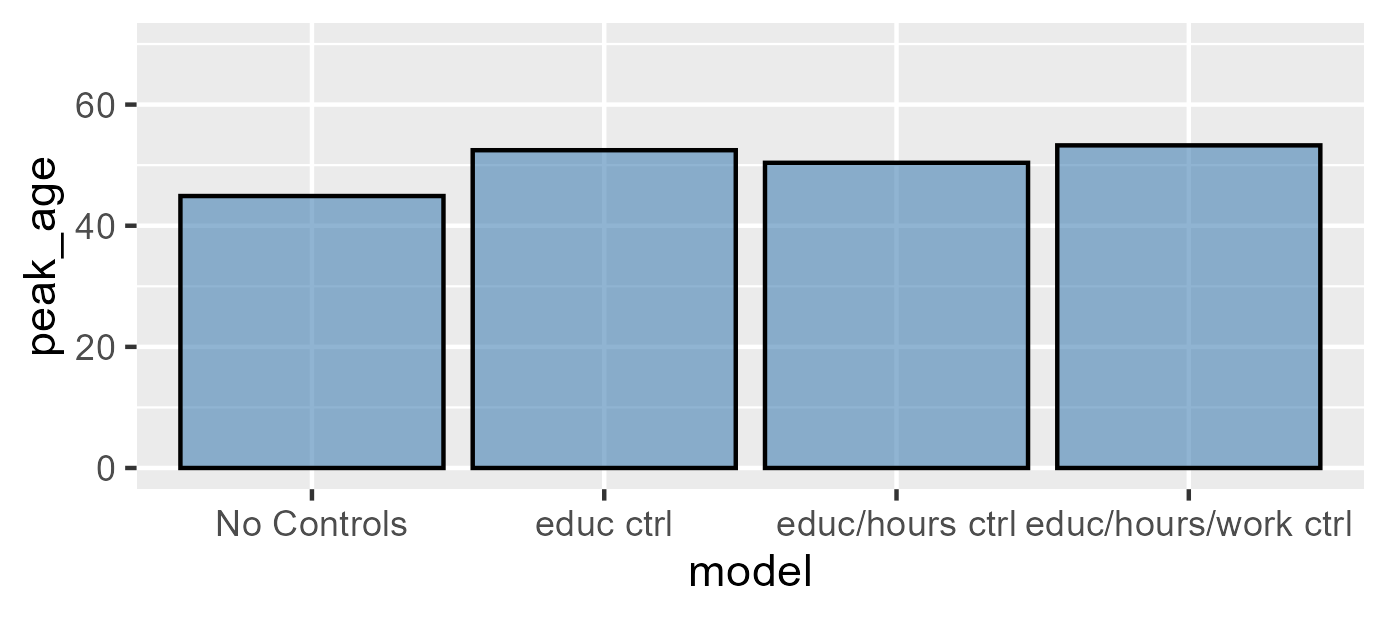
\includegraphics[scale=0.45]{../../views/age_peak_bar.png}
        \caption{Edad pico según modelos.}
    \end{figure}
    \column{0.5\textwidth}
    \begin{figure}
        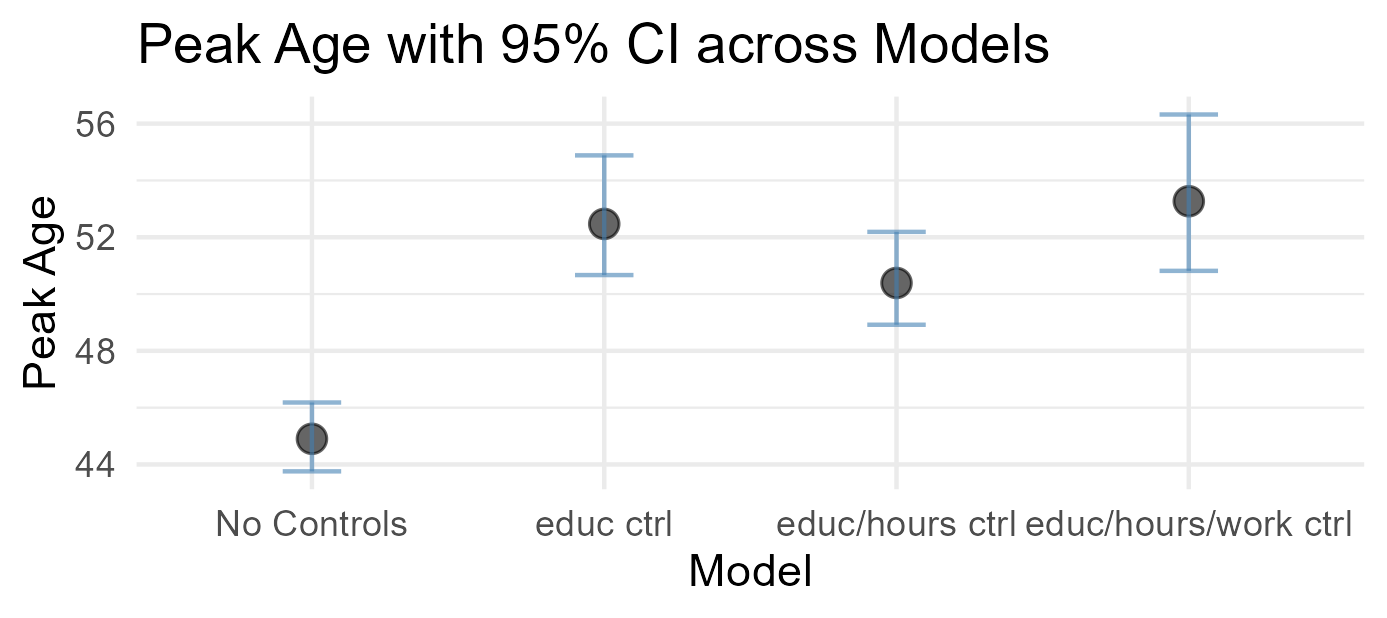
\includegraphics[scale=0.45]{../../views/age_whiskey_point.png}
        \caption{Intervalos de confianza (bootstrap).}
    \end{figure}
\end{columns}
\end{frame}
%---------------------

\end{document}